\documentclass[18pt,oneside,a4paper, titlepage]{article}

\usepackage[hidelinks]{hyperref}
\usepackage[pdftex]{graphicx}

\begin{document}
\begin{figure}[t]
	\centering
	
\includegraphics[scale=0.35]{logo-polimi.png}
\end{figure}
\title{\textbf{myTaxiService}\\\textbf{P}roject \textbf{P}lan \textbf{D}ocument\\ A.Y. 2015/2016\\
	Politecnico di Milano\\ Version 1.0}	
\author{Cattaneo Michela Gaia, matr. 791685\\Barlocco Mattia, matr. 792735 }
\date{February 2, 2016}
\maketitle

\newpage
\tableofcontents

\newpage
	\newpage
\section{Introduction}
	\subsection{Purpose}
		This document represents the Project Plan Document.\\ It specifies the effort and cost estimation of the myTaxiService project, by using the Function Points and COCOMO algorithmic techniques. Moreover, there is the explanation of the organization of the resources and of the tasks needed.\\
		The intended audience of this document is the project stakeholders and the development team.
	\subsection{Definitions and abbreviations}
		\begin{itemize}
			\item \textbf{Definitions}
			\item[-] \textbf{User}: a person who requests a service from the system. It can be a visitor or a passenger.
			\item[-] \textbf{Visitor}: a person who is not registered in the application.
			\item[-] \textbf{Passenger}: a person who is registered in the application.
			\item[-] \textbf{Taxi driver}: a taxi driver who access the application with a specific ID.
			\item[-] \textbf{Request}: the request of a taxi in a certain area and position in the city made by a user.
			\item[-] \textbf{Reservation}: the reservation of a taxi in a certain area, place and time that can be made only by passengers.
	
			\item \textbf{Acronyms and abbreviations}
			\item[-] \textbf{RASD}: Requirement Analysis and Specification Document
			\item[-] \textbf{DD}: Design Document
			\item[-] \textbf{JVM}: Java Virtual Machine
			\item[-] \textbf{FP}: Function Points
			\item[-] \textbf{COCOMO}: COnstructive COst MOdel
			\item[-] \textbf{ILF}: Internal Logic Files
			\item[-] \textbf{EIF}: External Interface Files
			\item[-] \textbf{KSLOC}: Kilo Source Lines Of Code
			\item[-] \textbf{EAF}: Effort Adjustment Factor
		\end{itemize}
	
	\newpage
	\subsection{Reference documents}
		\begin{itemize}
			\item Project Description and Rules (\url{https://github.com/MichelaCattaneo/myTaxiService/blob/master/Project\%20Description\%20And\%20Rules.pdf})
			\item Requirements Analysis and Specification Document (\url{https://github.com/MichelaCattaneo/myTaxiService/blob/master/Deliveries/RASD_1.1.pdf})
			\item Design Document (\url{https://github.com/MichelaCattaneo/myTaxiService/blob/master/Deliveries/DD.pdf})
			\item Code Inspection Document(\url{https://github.com/MichelaCattaneo/myTaxiService/blob/master/Deliveries/CodeInspection.pdf})
			\item Integration Test Document (\url{https://github.com/MichelaCattaneo/myTaxiService/blob/master/Deliveries/ITPD.pdf})
		\end{itemize}

\newpage
	\newpage
\section{Effort and Cost Estimation}
	%Apply Function Points to the project size and then COCOMO to estimate effort and cost

	\subsection{Function Points}
		Function points is part of the algorithmic techniques for cost and estimation modeling. It bases on the assumption that the dimension of software can be characterized by abstraction.\\
		This algorithmic technique is based on the complexity of five different entities: 
		\begin{itemize}
			\item number of input types: concern elementary operations that elaborate the data coming from the external environment.
			\item number of output types: concern elementary operations that generate the data for the external environment.
			\item number of inquiry types: concern input that controls the execution of the program and does not change the internal data structure, according to the query criteria.
			\item number of internal logic files (ILF): concern the internal data generated by the system.
			\item number of external interface files (EIF): concern the external interfaces to other systems or applications.
		\end{itemize}
		Their weights are showed in the table below.
		\vspace{0.9cm}
		\begin{center}
			\begin{tabular}{c c c c}
				\hline 	\textbf{Function Types} & & \textbf{Weight}  & \\[0.1cm]
				& Simple & Medium & Complex\\[0.1cm]
				\hline	N. Inputs & 3 & 4 & 6 \\[0.05cm]
				\hline	N. Outputs & 4 & 5 & 7 \\[0.05cm]
				\hline	N. Inquiry & 3 & 4 & 6 \\[0.05cm]
				\hline	N. ILF & 7 & 10 & 15 \\[0.05cm]
				\hline	N. EIF & 5 & 7 & 10 \\[0.05cm]
				\hline
			\end{tabular}
		\end{center}
		\newpage
		\subsubsection{External Inputs}
			The system allows the customer or the taxi driver to:
			\begin{itemize}
				 \item Sign up
				 \item Log in and log out
				 \item Request a taxi
				 \item Reserve a taxi
				 \item Choose the payment method
				 \item Manage the profile
				 \item Change status
				 \item Answer to taxi requests
			\end{itemize}
			All of these operations are rather simple and involves at most two entities, so a simple weight can be adopted.
			\begin{center}
				\textbf{Inputs: 9 x 3 = 27 FPs}
			\end{center}
		\subsubsection{External Outputs}
			The system sends to the customer information about the taxi driver arrival, after the request and to the taxi driver his position in the queue and the request notification.\\
			The first two entities are complex, as they should get some information both from the ILF and the EIF, so a complex weight will be adopted. While for the request notification it is necessary to get information from two tables of the ILF, so it can be considered a medium complexity.
			\begin{center}
				\textbf{Outputs: 2 x 7 + 1 x 5 = 19 FPs}
			\end{center}
		\subsubsection{External Inquiry}
			The system allows the users and the taxi drivers to see their profile, which can be consider a simple information request.\\The passenger in particular can also see his previous requests and the taxi driver can see his position in the queue of his area and the previous notifications. The visualization of the position can be considered simple, while the visualization of the requests and notification requires to load a more consistent amount of data, so they will be considered medium weighted.
			\begin{center}
				\textbf{Inquiries: 2 x 3 + 2 x 4 = 14 FPs}
			\end{center}
		\newpage
		\subsubsection{ILF}
			The application stores information about:
			\begin{itemize}
				\item passenger
				\item taxi driver
				\item city area
				\item request
				\item reservation
			\end{itemize}
			All these entities has a simple structure in a database, in fact their table is composed of a few fields. Therefore we can decide to use a simple weight for all of them except for the city area table that can be considered of medium complexity because it has to store also the information about the taxi queues.
			\begin{center}
				\textbf{ILF: 4 x 7 + 1 x 10= 38 FPs}
			\end{center}
		\subsubsection{EIF}
			The application manages the interaction with three external systems:
			\begin{itemize}
				\item Google Maps, in order to determine the position of the taxi drivers and of the users.
				\item Facebook, in order to get the user personal information if he wants to log in with his Facebook account.
				\item Google+, in  order to get the user personal information if he wants to log in with his Google+ account.
			\end{itemize}
			The position of all the different users can be considered a medium complexity entity, so we will adopt a medium weight. As regards the other two entities about the personal information, they can be considered simple weighted, as they have a simple structure.\\
			\begin{center}
				\textbf{EIF: 1 x 7 + 2 x 5 = 17 FPs}
			\end{center}
		\subsubsection{Result}
			The total number of function points is:
			\vspace{0.5cm}
			\begin{center}
				\begin{tabular}{c c c c}
					\hline 	\textbf{Function Types} &	&	& \textbf{FPs} \\[0.1cm]
					\hline	N. Inputs & & & 27 \\[0.05cm]
						N. Outputs & & & 19  \\[0.05cm]
						N. Inquiry & & & 14  \\[0.05cm]
						N. ILF & & & 38  \\[0.05cm]
						N. EIF & & & 17  \\[0.05cm]
					\hline Total FPs & & & 115\\[0.05cm]
					\hline
				\end{tabular}
			\end{center}
			\vspace{0.5cm}
	\newpage
	\subsection{COCOMO}
		COCOMO is a cost estimation model. It is based on the function points previously calculated and on the lines of code of the project, that, along with the scale drivers, help to determine the general effort, duration and number of people needed for the project.\\
		In order to calculate the Source Lines Of Code (SLOC), it necessary to know how much SLOC per FP are needed in average for a J2EE project. This information can be found on the QSM website (\url{http://www.qsm.com/resources/function-point-languages-table}), where we can find the factor 46. Therefore the estimated number of lines of code is:
		\vspace{0.5cm}	
		\begin{center}
			\begin{math}
				SLOC = FP * 46 = 115 * 46 = 5290
			\end{math}
		\end{center}
		\vspace{0.5cm}
		We can consider the “Nominal” values of Cost Drivers (EAF = 1.00) and Scale Drivers (E = 1.0997) in order to calculate the effort, inserting this values in the formula:
		\vspace{0.5cm}
		\begin{center}
			\begin{math}
				effort = 2.94*EAF*(KSLOC)^{E}
			\end{math}
		\end{center}
		\begin{center}
			\begin{math}
				effort = 2.94*1.00*(5.29)^{1.0997} = 18.36 Person/months
			\end{math}
		\end{center}
		\vspace{0.5cm}
		The duration of the project can be found with this formula, considering the exponent E = 0.3179:
		\vspace{0.5cm}
		\begin{center}
			\begin{math}
				Duration = 3.67*(effort)^{E}
			\end{math}
		\end{center}
		\begin{center}
			\begin{math}
				Duration = 3.67*(18.36)^{0.3179} = 9.25 Months
			\end{math}
		\end{center}
		\vspace{0.5cm}
		Now it is possible to calculate	the number of people needed for this project.
		\vspace{0.5cm}
		\begin{center}
			\begin{math}
				N. people = effort / Duration
			\end{math}
		\end{center}
		\begin{center}
			\begin{math}
				N. people = 18.36 / 9.25 = 1.98 people
			\end{math}
		\end{center}
		\vspace{0.5cm}
	\subsection{Conclusions}
		In the Function Points part, we have overestimated some weight of the entities in order to reach an estimation that allows to finish in time or before the expected time. As regards the COCOMO results, the number of people coincide with the reality and the duration of the project is reasonable, tho maybe it is overestimated, as said before, and it is possible to reduce it.
\newpage
\section{Task Scheduling}
	Here is presented a list of the relevant tasks of the project, with their schedule, dependencies and the time spent for each one:
	\begin{itemize}
		\item \textbf{T1} RASD: this is the first task to accomplish. It describes the most important features of the project: requirements, assumptions, interfaces, model of the Database and how the myTaxiService application should work. It is necessary to redact and finish this document, identifying all the essential aspects, before it is possible to start the project.\\ \textit{Estimated time: about 10 days}.\\ \textit{Dependencies: -}.
		\item \textbf{T2} Design Document: this document describes the architectural design of the myTaxiService system. It is also part of the documentation necessary to finish before the project starts. In facts, after the RASD has been done, it is necessary to identify the architecture and the components of the project, before actually starting to code.\\ \textit{Estimated time: about 10 days}.\\ \textit{Dependencies: T1}.
		\item \textbf{T3} Database: based on the model described in the RASD and in the Design Document, this task consists in the creation of the tables of the database.\\ \textit{Estimated time: about 15 days}.\\ \textit{Dependencies: T2}.
		\item \textbf{T4} Interfaces: based on the interfaces shown in the RASD and in the Design Document, this task contains the code implementing the interfaces on the client side.\\ \textit{Estimated time: about 2 months}.\\ \textit{Dependencies: T2}.
		\item \textbf{T5} Requirements: this task consists in the development of the application logic on the server side (for example the AccessManager component that manages the login and the registration or the RequestManager that manages requests,  reservations and notifications).\\ \textit{Estimated time: about 2 months}.\\ \textit{Dependencies: T3}.
		\item \textbf{T6} Code Inspection: once the code part is completed, it is necessary to check that the code is bug free, also verifying that all the coding conventions are respected, in order to improve its quality and, in the meantime, to assure that there are no issues.\\ \textit{Estimated time: about 1 month}.\\ \textit{Dependencies: T4,T5}.
		\item \textbf{T7} Code Inspection Document: once the code inspection is done, it is necessary to document any issue found in the code.\\ \textit{Estimated time: 5 days}.\\ \textit{Dependencies: T6}.
		\item \textbf{T8} Test Document: this task consists of the redaction of a document that explains the strategy adopted for unit testing, integration testing and system testing. This must be done after the code is completed and before the actual testing.\\ \textit{Estimated time: about 10 days}.\\ \textit{Dependencies: T6}.
		\item \textbf{T9} Unit Testing: according to what is written in the Test Document, this task involves accomplishing the unit testing.\\ \textit{Estimated time: about 20 days}.\\ \textit{Dependencies: T8}.
		\item \textbf{T10} Integration Testing: according to what is written in the Test Document, this task involves accomplishing the integration testing.\\ \textit{Estimated time: about 20 days}.\\ \textit{Dependencies: T8}.
		\item \textbf{T11} System Testing: according to what is written in the  Test Document, this task involves accomplishing the system testing.\\ \textit{Estimated time: about 20 days}.\\ \textit{Dependencies: T9,T10}.
	\end{itemize}
	The project should start on October 2015 and, according to the time estimation and the resource allocation, it should be over in about 6 months on March 2016. Comparing this assumption with the COCOMO results, that states that the project should last 9 months, the reality could reasonably be in the middle of this two estimation.\\ \\ This is a simple Gantt chart of the task schedule:\\
	\vspace{0.5cm}
	\begin{center}
	\centering
	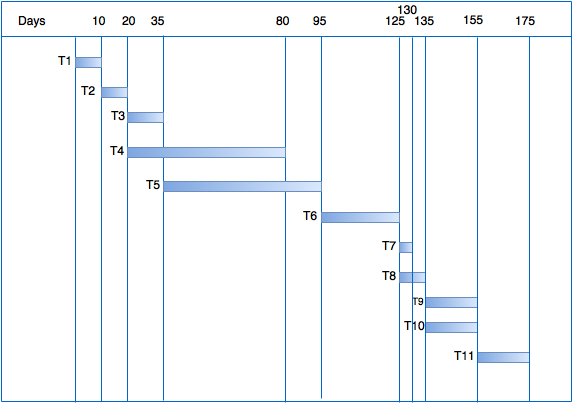
\includegraphics[scale=0.57]{scheduleTask.png}
	\end{center}
	% Identify the tasks for your project and their schedule. Do so retrospectively, assuming that the project has started in October 2015, as it really happened.
	
\newpage
\section{Resources Allocation}
	\vspace{0.8cm}
	\begin{center}
		\centering
		\begin{tabular}{c c c }
			\hline \textbf{Task} & \textbf{Effort(person)} & \textbf{Dependencies} \\[0.1cm]
			\hline		T1 & 2 & -\\[0.1cm]
			\hline		T2 & 2 & T1\\[0.1cm]
			\hline		T3 & 1 & T2\\[0.1cm]
			\hline		T4 & 1 & T2\\[0.1cm]
			\hline		T5 & 1 & T3\\[0.1cm]
			\hline		T6 & 2 & T4,T5\\[0.1cm]
			\hline		T7 & 1 & T6\\[0.1cm]
			\hline		T8 & 1 & T6\\[0.1cm]
			\hline		T9 & 1 & T8\\[0.1cm]
			\hline		T10 & 1 & T8\\[0.1cm]
			\hline		T11 & 2 & T10,T9\\[0.1cm]
			\hline
		\end{tabular}
	\end{center}
	\vspace{0.8cm}
	Based on the schedule and the availability of our resources, the members of the team can be allocated to the tasks in this way:
	\begin{itemize}
		\item \textbf{T1}: we can allocate all the resources (two people) to this task because without it we cannot start the next tasks. In fact the resources are allocated to the redaction of the RASD in order to accelerate its completion and therefore start as soon as possible the other tasks.
		\item \textbf{T2}: we allocate all the resources (two people) to the redaction of the Design Document because it is necessary to complete the architectural design before continuing with the project development.
		\item \textbf{T3}: we can allocate one person to the creation of the database after the task T2.
		\item \textbf{T4}: we can allocate one person to the development of the interfaces during the creation of the database, because this task does not need the database implementation part.
		\item \textbf{T5}: we can allocate one person to the development of the server side of the system (requirements). The person that we allocate to this task is the same that we allocated to the task 3 because this task needs a database to be developed.
		\item \textbf{T6}: once T4 and T5 are done, we allocate the two people in the team to this task because it requires a good deal of time and its duration can be reduced with two people.
		\newpage
		\item \textbf{T7}: after T6, we allocate one person to redact the Code Inspection Document.
		\item \textbf{T8}: after T6 and during T7, we can allocate the other person to write the Test Document.
		\item \textbf{T9}: after T8, we allocate one person to write unit tests.
		\item \textbf{T10}: during T9, the other person can be allocated to the integration test.
		\item \textbf{T11}: once T9 and T10 are done, we allocate all the resources for the system test.
	\end{itemize}
	% Allocate the resources (all memebers of your group) to the various tasks. In defining the allocation, take into account your actual availability for the project.

\newpage
	\newpage
\section{Risks and Recoveries}
	% Define the risks for the project, their relevance and the associated recovery actions.
	Risk management is an important issue for the development of a project, as long as the risks can affect the project schedule or the quality of the product, increasing the costs and efforts that were previously estimated. \\ The strategy adopted is the proactive strategy, that follows fixed steps in order to manage the issues in advance. The first step consists in identifying potential problems and threats the product can be subject to. Then it is necessary to determine the recovery actions and all the ways to reduce the risks.\\ These are the risks that could be found:
	\begin{itemize}
		\item \textbf{Project risk.} This is a critical risk: it is possible that, going on in the implementation of the system, the requirements unexpectedly grows with respect to the one identified at the beginning. So it could be difficult to follow the project schedule and therefore the product is finished later than the estimated time. This will imply an increase in the efforts and in the costs.\\ In order to avoid this kind of problem, which has a high relevance, it is necessary to monitor every phase of the project, comparing it with existing projects. In case this is not enough, it can always be possible to release an early version of the project with less functionalities and then, when possible, release the complete version.
		\item \textbf{Market risk}. It is possible that, even though the project is good and efficient, it is difficult to sell because it is not what people needs in that moment, for example if there is already a similar product on the market.\\ There is not a real strategy to adopt against this kind of risks, in fact it is quite unpredictable and it depends on the market trends. In order to at least try to reduce the possibility of this kind of situations a study on the market could help.
		\item \textbf{Technology to be built.} This is a relevant risk relied to the technological part of the application: the most critical issues for an application like myTaxiService, that should be reliable and responsive, are data loss and performance issues.\\ In order to avoid the deterioration of the service, a particular care on this aspect must be taken in account. The server should always be on and available, in order to compute all the requests in a short amount of time and the algorithms computing the taxi queues and the taxi positioning should be implemented in the most efficient ways. In particular, to prevent data loss, the functioning protocol for the client-server data transmission should be adopted.
		\item \textbf{Staff experience.} It is possible that the lack of technical experience of the project developers affect the quality of the software and the schedule of the project.\\ In order to prevent this from happening it is necessary that the group is guided by someone with more experience or that the developers are able to follows existing guidelines of previous projects. This is not a really relevant risk, as the project developers can always take into account previous projects and material.
	\end{itemize}
\newpage
\section{Appendix}

	\subsection{Software and tool used}
		\begin{itemize}
			\item TeXstudio (\url{http://www.texstudio.org/}): to redact and to format this document.
		\end{itemize}
	
	\subsection{Hours of work}
		Time spent redacting this document:
		\begin{itemize}
			\item Cattaneo Michela Gaia: {\raise.17ex\hbox{$\scriptstyle\sim$}}12 hours of work.
			\item Barlocco Mattia: {\raise.17ex\hbox{$\scriptstyle\sim$}}12 hours of work.
		\end{itemize}

\end{document}